\begin{figure}[h]
    \centering
    \begin{subfigure}[b]{0.56\textwidth}
        \centering
        \caption{}
        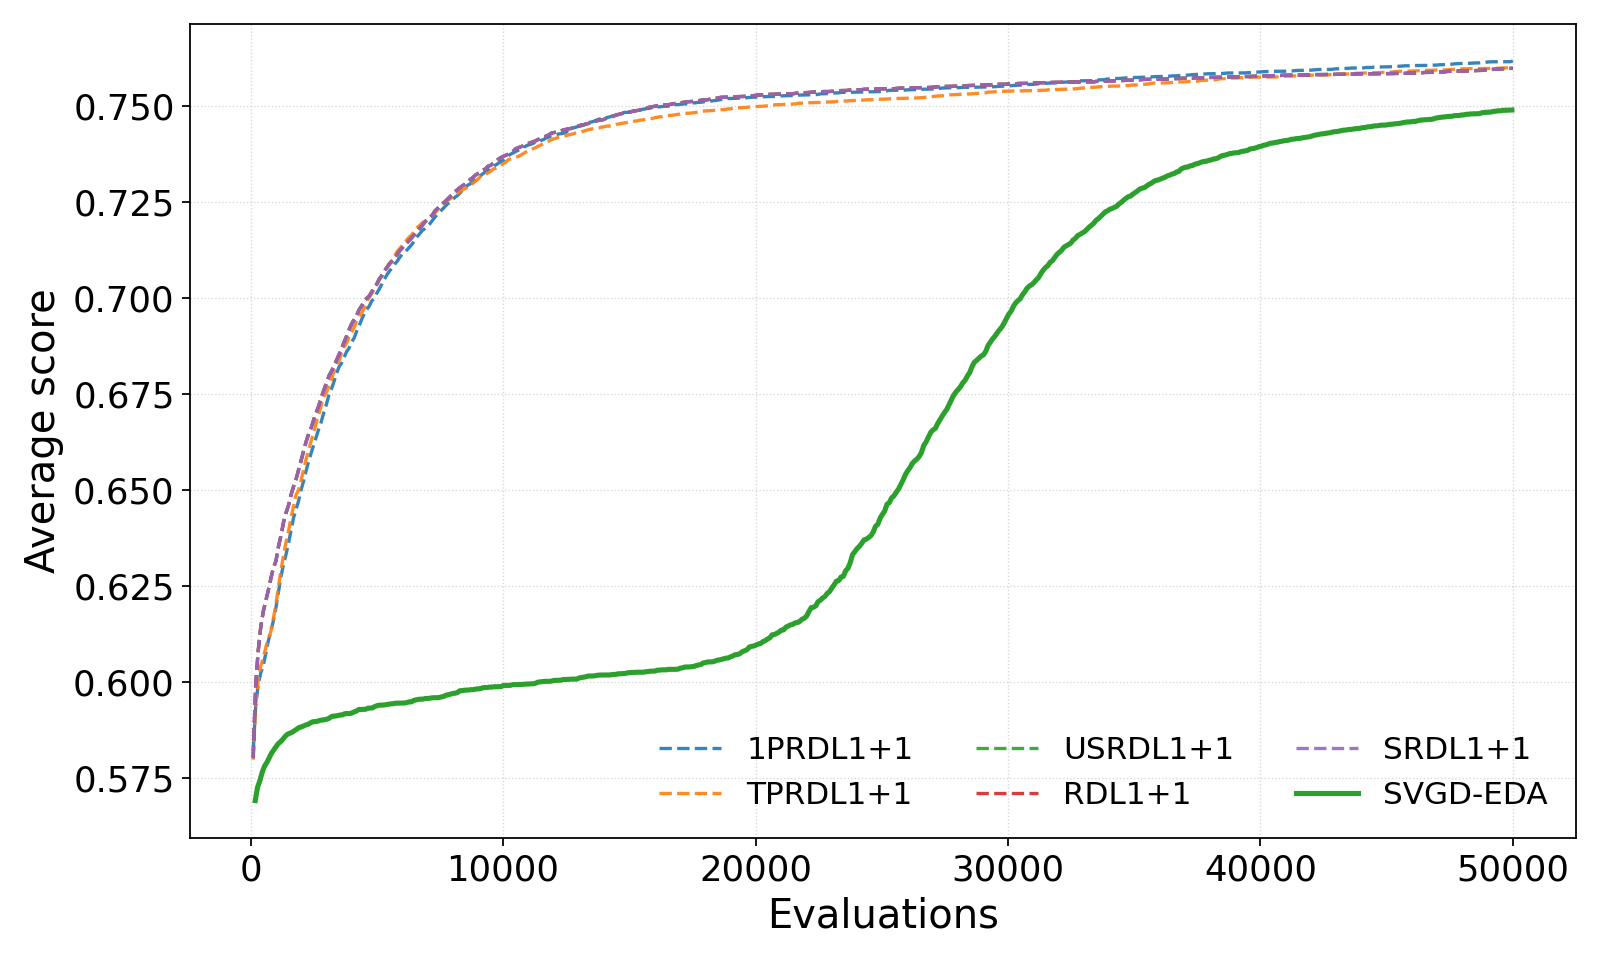
\includegraphics[width=\linewidth]{comparison_nk3_128_t8.png}
        \label{fig:comparison_nk3_128_t8}
    \end{subfigure}
    \vspace{0.5cm}
    \begin{subfigure}[b]{0.42\textwidth}
        \centering
        \caption{}
        
\includegraphics[width=\linewidth]{boxplot_final_score_vs_top5.png}
        \label{fig:boxplot_nk3_128_t8}
    \end{subfigure}

    \caption{Performance analysis on a NK3 instance distribution ($n=128, K=8$). (a) Evolution of the average score for \texttt{SVGD-EDA} and the top-five competitors. (b) Final score distribution after 50,000 evaluations. Both panels use the same labels/colors: SVGD-EDA, 1PRDL1+1, TPRDL1+1, USRDL1+1, RDL1+1, SRDL1+1. Acronyms in legends: 1PRDL1+1 = \texttt{OnePtRecombiningDiscreteLenglerOnePlusOne}; TPRDL1+1 = \texttt{TwoPtRecombiningDiscreteLenglerOnePlusOne}; USRDL1+1 = \texttt{UltraSmoothRecombiningDiscreteLenglerOnePlusOne}; RDL1+1 = \texttt{RecombiningDiscreteLenglerOnePlusOne}; SRDL1+1 = \texttt{SmoothRecombiningDiscreteLenglerOnePlusOne}.}
    \label{fig:benchmark_plots_nk3_128_t8}
\end{figure}
